%        File: coordination.tex
%     Created: Wed Oct 28 05:00 PM 2015 C
% Last Change: Wed Oct 28 05:00 PM 2015 C
%
\documentclass{standalone}

\usepackage{tikz}
\usetikzlibrary{positioning, shapes, calc, backgrounds, fit}

\begin{document}
\begin{tikzpicture}[align = center, font = \Huge]
  \node (lock) [label = -90 : {Distributed Lock}] {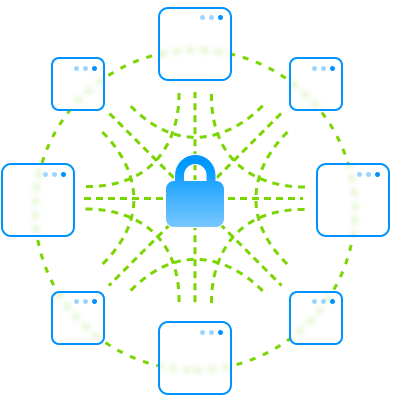
\includegraphics[scale = 
  0.50]{figures/distributed-lock-icon.png}};
  \node (member) [right = 1.5cm of lock, label = -90 : {Group Membership}] {
\includegraphics[scale = 
  2.00]{figures/membership-icon.png}};
  \node (leader) [right = 1.5cm of member, label = -90 : {Leader Election}] {
\includegraphics[scale = 
  0.75]{figures/ring-computer-icon.png}};
  \node (queue) [right = 1.5cm of leader, label = -90 : {Queue Service}] {
\includegraphics[scale = 
  0.15]{figures/amazon-sqs-icon.png}};

  \draw [very thick, blue] ($(lock.south) + (0.0cm, -2.0cm)$) to ++(24.0cm, 0.0cm);

  \node (zookeeper) [below right = 4.0cm and 1.0cm of lock.south west] {
\includegraphics[scale = 
  0.60]{figures/apache-zookeeper.png}};
  \node (chubby) [right = 3.0cm of zookeeper] {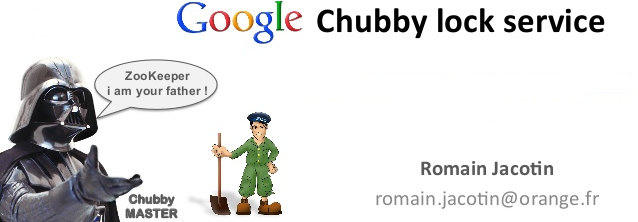
\includegraphics[scale = 
  0.60]{figures/chubby-google-logo.png}};


  % \node (jigsaw) [right = 1.5cm of leader, label = -90 : {Multi-party Jigsaw}] {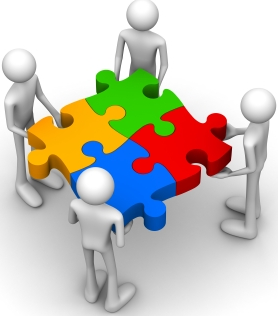
\includegraphics[scale = 
  % 0.45]{figures/jigsaw-icon.png}};
\end{tikzpicture}
\end{document}


